\documentclass{article}
\usepackage{amsmath}
\usepackage{tikz}
\usetikzlibrary{arrows}
\begin{document}

\section*{Independence and Factoring}
Let $A$, $B$, $C$, and $D$ be binary valued random variables that take
on the values 1 or 0.

These variables can take on $2^4$ permutations. In general, if we are
interested in the probability of any these permutations we need to
keep track of sixteen separate values.

\begin{align*}
&\Pr(A=0,B=0,C=0,D=0) = P_1 \\
&\Pr(A=1,B=0,C=0,D=0) = P_2 \\
&\Pr(A=0,B=1,C=0,D=0) = P_3 \\
&\vdots \\
&\Pr(A=1,B=1,C=0,D=1) = P_{14} \\
&\Pr(A=1,B=1,C=1,D=0) = P_{15} \\
&\Pr(A=1,B=1,C=1,D=1) = P_{16} 
\end{align*}

If these variables are independent, then we only need to know four
values -- the probability of each random variable taking a value. 

Independence means that the probability of realizing a permutation of
values factors into the product of each value taking on the
corresponding value.

\begin{equation}
\Pr(A,B,C,D) = \Pr(A)\Pr(B)\Pr(C)\Pr(D)
\end{equation}

We can represent the dependence and independence relations between random
variables in a graph. If the four variables are independent, then we draw
the variables as nodes with edges between them.


\begin{figure}[!ht]
\centering
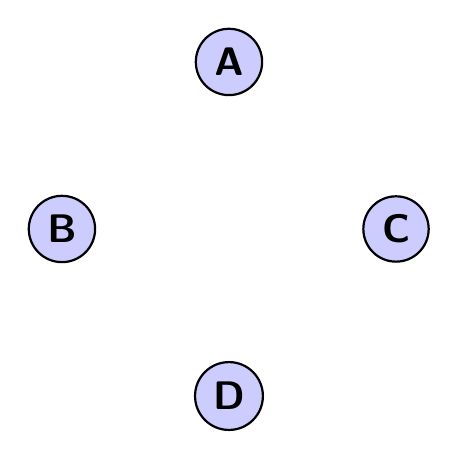
\begin{tikzpicture}[->,>=stealth',shorten >=1pt,auto,node distance=3cm,
  thick,main node/.style={circle,fill=blue!20,draw,font=\sffamily\Large\bfseries}]

  \node[main node] (1) {A};
  \node[main node] (2) [below left of=1] {B};
  \node[main node] (3) [below right of=2] {D};
  \node[main node] (4) [below right of=1] {C};


\end{tikzpicture}
\caption{Completely Independent Variables}
\end{figure}

If each variable is dependent on all the others, then the graph is
completely connected.

\begin{figure}
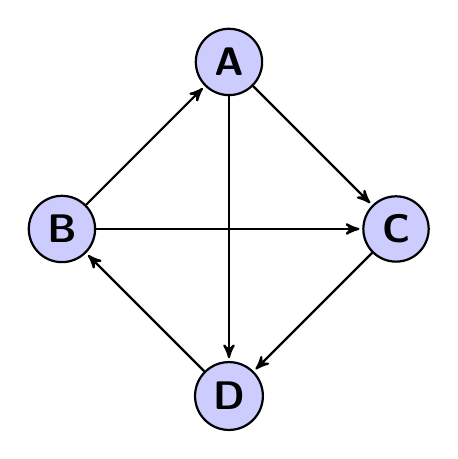
\begin{tikzpicture}[->,>=stealth',shorten >=1pt,auto,node distance=3cm,
  thick,main node/.style={circle,fill=blue!20,draw,font=\sffamily\Large\bfseries}]

  \node[main node] (1) {A};
  \node[main node] (2) [below left of=1] {B};
  \node[main node] (3) [below right of=2] {D};
  \node[main node] (4) [below right of=1] {C};

  \path[every node/.style={font=\sffamily\small}]
    (1) edge node [left] {} (4)
        edge node [left] {} (3)
    (2) edge node [right] {} (1)
        edge node {} (4)
    (3) edge node [right] {} (2)
    (4) edge node [left] {} (3);
\end{tikzpicture}
\end{figure}

\end{document}